\documentclass[10pt]{beamer}

% Beamer style
%\usetheme[secheader]{Madrid}
\usetheme{CambridgeUS}
\usecolortheme[rgb={0.65,0.15,0.25}]{structure}
%\usefonttheme[onlymath]{serif}
\beamertemplatenavigationsymbolsempty
%\AtBeginSubsection

% Packages
%\usepackage[french]{babel}
\usepackage[latin1]{inputenc}
\usepackage{color}
\usepackage{xspace}
%\usepackage{dsfont, stmaryrd}
\usepackage{amsmath, amsfonts, amssymb}
\usepackage{epsfig}
\usepackage{url}
\usepackage{/home/robin/LATEX/Biblio/astats}
%\usepackage[all]{xy}
\usepackage{graphicx}

% Commands
\definecolor{darkred}{rgb}{0.65,0.15,0.25}
%\newcommand{\emphase}[1]{\textcolor{darkred}{#1}}
\newcommand{\emphase}[1]{{#1}}
\newcommand{\paragraph}[1]{\textcolor{darkred}{#1}}
\newcommand{\refer}[1]{{\footnotesize{\textcolor{gray}{{[\cite{#1}]}}}}}
\newcommand{\Refer}[1]{{\footnotesize{\textcolor{gray}{[{#1}]}}}}
\renewcommand{\newblock}{}

% Symbols
\newcommand{\Abf}{{\bf A}}
\newcommand{\Beta}{\text{B}}
\newcommand{\Bcal}{\mathcal{B}}
\newcommand{\BIC}{\text{BIC}}
\newcommand{\Ccal}{\mathcal{C}}
\newcommand{\dd}{\text{~d}}
\newcommand{\dbf}{{\bf d}}
\newcommand{\Dcal}{\mathcal{D}}
\newcommand{\Esp}{\mathbb{E}}
\newcommand{\Ebf}{{\bf E}}
\newcommand{\Ecal}{\mathcal{E}}
\newcommand{\Gcal}{\mathcal{G}}
\newcommand{\Gam}{\mathcal{G}\text{am}}
\newcommand{\Hcal}{\mathcal{H}}
\newcommand{\Ibb}{\mathbb{I}}
\newcommand{\Ibf}{{\bf I}}
\newcommand{\ICL}{\text{ICL}}
\newcommand{\Cov}{\mathbb{C}\text{ov}}
\newcommand{\Corr}{\mathbb{C}\text{orr}}
\newcommand{\Var}{\mathbb{V}}
\newcommand{\Vsf}{\mathsf{V}}
\newcommand{\pen}{\text{pen}}
\newcommand{\Fcal}{\mathcal{F}}
\newcommand{\Hbf}{{\bf H}}
\newcommand{\Jcal}{\mathcal{J}}
\newcommand{\Kbf}{{\bf K}}
\newcommand{\Lcal}{\mathcal{L}}
\newcommand{\Mcal}{\mathcal{M}}
\newcommand{\mbf}{{\bf m}}
\newcommand{\mum}{\mu(\mbf)}
\newcommand{\Ncal}{\mathcal{N}}
\newcommand{\Nbf}{{\bf N}}
\newcommand{\Nm}{N(\mbf)}
\newcommand{\Ocal}{\mathcal{O}}
\newcommand{\Obf}{{\bf 0}}
\newcommand{\Omegas}{\underset{s}{\Omega}}
\newcommand{\Pbf}{{\bf P}}
\newcommand{\Pt}{\widetilde{P}}
\newcommand{\Pcal}{\mathcal{P}}
\newcommand{\Qcal}{\mathcal{Q}}
\newcommand{\Rbb}{\mathbb{R}}
\newcommand{\Rcal}{\mathcal{R}}
\newcommand{\Scal}{\mathcal{S}}
\newcommand{\Ucal}{\mathcal{U}}
\newcommand{\Vcal}{\mathcal{V}}
\newcommand{\BP}{\text{BP}}
\newcommand{\EM}{\text{EM}}
\newcommand{\VEM}{\text{VEM}}
\newcommand{\VBEM}{\text{VBEM}}
\newcommand{\cst}{\text{cst}}
\newcommand{\obs}{\text{obs}}
\newcommand{\ra}{\emphase{\mathversion{bold}{$\rightarrow$}~}}
%\newcommand{\transp}{\text{{\tiny $\top$}}}
\newcommand{\transp}{\text{{\tiny \mathversion{bold}{$\top$}}}}
\newcommand{\logit}{\text{logit}\xspace}

% Directory
\newcommand{\figmixt}{/home/robin/ENSEIGN/COURS/MELANGE}
\newcommand{\figbma}{/home/robin/RECHERCHE/RUPTURES/MELANGE/Exemples/Grippe}
\newcommand{\fignet}{../FIGURES}
\newcommand{\figeco}{/home/robin/RECHERCHE/ECOLOGIE/EXPOSES/FIGURES}
%\newcommand{\figmotif}{/home/robin/RECHERCHE/RESEAUX/Motifs/FIGURES}


%====================================================================
%====================================================================

%====================================================================
%====================================================================
\begin{document}
%====================================================================
%====================================================================

%====================================================================
\title[Network analysis using $W$-graphs]{Network analysis with the $W$-graph model \\ {\large (via the Stochastic Block Model)}}

\author{S. Robin \\ ~\\
  Joint work with P. Latouche and S. Ouadah}

\institute[INRA / AgroParisTech]{INRA / AgroParisTech \\
  \vspace{-.1\textwidth}
  \begin{tabular}{ccccc}
    
\includegraphics[height=.3\textheight]{\fignet/LogoINRA-Couleur} & 
    \hspace{.02\textheight} &
    
\includegraphics[height=.08\textheight]{\fignet/logagroptechsolo} & 
    \hspace{.02\textheight} &
    
\includegraphics[height=.09\textheight]{\fignet/logo-ssb}
    \\ 
  \end{tabular} \\
  \bigskip
  }

\date[IMS, Singapore]{IMS, June 2015, Singapore}

%====================================================================
%====================================================================
\maketitle
%====================================================================

%====================================================================
\frame{\frametitle{Outline}
  \tableofcontents
  }
%====================================================================

%====================================================================
%====================================================================
\section{Modeling heterogeneity in interaction networks}
%====================================================================
\frame{\frametitle{Modeling heterogeneity in (biological) interaction networks}}

%====================================================================
\subsection*{Heterogeneity in biological networks}
%====================================================================
\frame{\frametitle{Heterogeneity in biological networks} 

  Biological networks describe interactions between entities: genes, proteins, individuals, species... \\
  ~\\
  Observed networks display heterogeneous topologies, that one would like to decipher and better understand. \\
  ~\\

  \pause
    \begin{tabular}{ll}
    %\hspace{-.02\textwidth}
    \begin{tabular}{p{.5\textwidth}}
      \paragraph{Dolphine social network.} \\
      \includegraphics[width=.4\textwidth]{../FIGURES/NeG04-Fig11} \\
      \refer{NeG04}
    \end{tabular}
    & 
    \hspace{-.02\textwidth}
    \begin{tabular}{p{.5\textwidth}}
      \paragraph{{\sl H. pylori} PPI network.} \\
      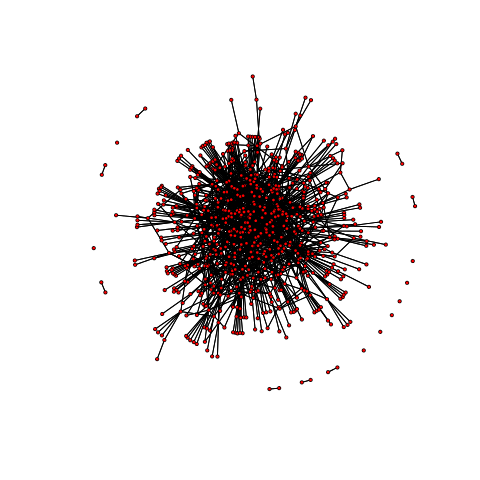
\includegraphics[width=.4\textwidth]{../FIGURES/Hpylo20060402-graph}
    \end{tabular} 
  \end{tabular} 
  }

%====================================================================
\frame{\frametitle{Heterogeneous means ...} 

  \paragraph{... not homogeneous,} that is to say: different from an Erd�s-Renyi (ER) graph.
  
  \bigskip \bigskip 
  \paragraph{Erd�s-Renyi random graph $\Gcal(n, p)$:} Consider $n$ nodes, node pairs $1 \leq i < j \leq n$ are independently connected with same probability $p$:
  $$
  (Y_{ij}) \text{ iid, } \qquad Y_{ij} \sim \Bcal(p).
  $$
  
  \bigskip
  \begin{itemize}
   \item Very intensively studied.
   \item Fits very few real-life networks.
  \end{itemize}

}

%====================================================================
\subsection*{Latent space models}
%====================================================================
\frame{\frametitle{Latent space models}

  \paragraph{Latent variables} allow to capture some underlying structure of a network (see review \Refer{Matias and R. (2014)}\nocite{MaR14}).

  \bigskip \bigskip \pause
  \paragraph{General setting for binary graphs.} \refer{BJR07}: %\pause
  \begin{itemize}
   \item   \emphase{A latent (unobserved) variable $Z_i$} is associated with each node:
  $$
  \{Z_i\} \text{ iid } \sim \pi 
  $$
  \item 
  Edges \emphase{$Y_{ij} = \Ibb\{i \sim j\}$ are independent conditionally} to the $Z_i$'s:
  $$
  \{Y_{ij}\} \text{ independent } | \{Z_i\}: \Pr\{Y_{ij} = 1\} = \gamma(Z_i, Z_j)
  $$
  \end{itemize}

  \bigskip \pause
  \paragraph{We focus here on model approaches}, in contrast with, e.g.
  \begin{itemize}
  \item Graph clustering \refer{GiN02}, \refer{New04}; 
  \item Spectral clustering \refer{LBB08}.
  \end{itemize}

}

%====================================================================
\frame{\frametitle{Latent space models}

  \vspace{-.2\textheight}
  \begin{tabular}{cc}
  \vspace{-.3\textheight}
  \hspace{-.05\textwidth}
    \begin{tabular}{p{.5\textwidth}}
      \onslide+<1->{
	\paragraph{State-space model: principle.}}
	 \begin{itemize}
	   \onslide+<2->{
        \item Consider $n$ nodes ($i = 1..n$); \\ ~ } 
        \onslide+<3->{
        \item $Z_i = $ unobserved position of node $i$, e.g.
          $$
          \{Z_i\} \text{ iid } \sim \Ncal(0 ,I)
          $$} 
        \onslide+<4->{
        \item Edge $\{Y_{ij}\}$ independent given $\{Z_i\}$, e.g.
          $$
          \Pr\{Y_{ij} = 1\} = \gamma(Z_i, Z_j).
          $$}
      \end{itemize}
    \end{tabular}
    & 
    \hspace{-.05\textwidth}
    \begin{tabular}{p{.5\textwidth}}
      \vspace{.05\textheight}
      \begin{overprint}
        \onslide<3>
        \hspace{-.05\textwidth}
        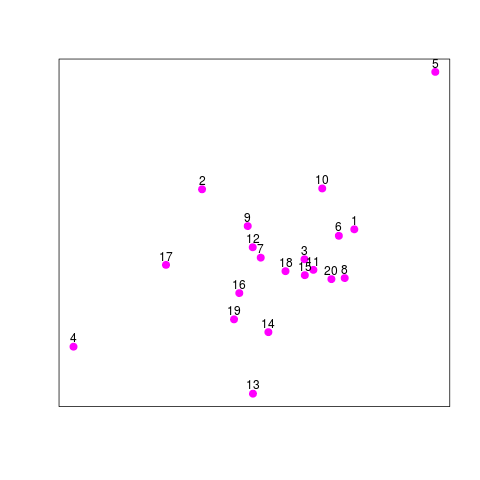
\includegraphics[width=.5\textwidth]{\fignet/FigCLADAG-LPM-Y}    
        \onslide<4>
        \hspace{-.05\textwidth}
        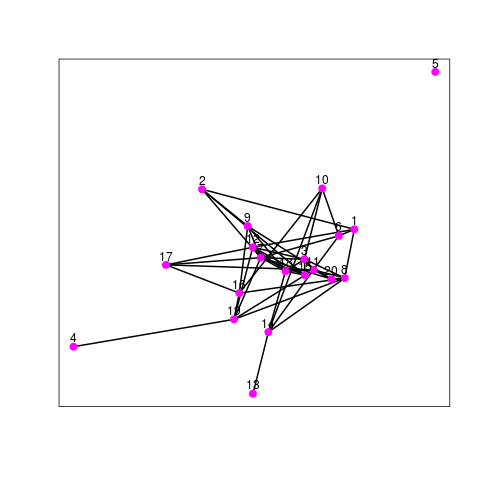
\includegraphics[width=.5\textwidth]{\fignet/FigCLADAG-LPM-XY}    
        \onslide<5>
%         \hspace{-.05\textwidth}
%         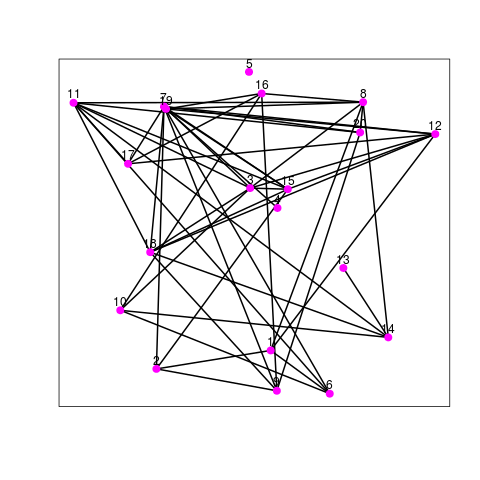
\includegraphics[width=.5\textwidth]{\fignet/FigCLADAG-LPM-X1}    
%         \onslide<6>
%         \hspace{-.06\textwidth}
%         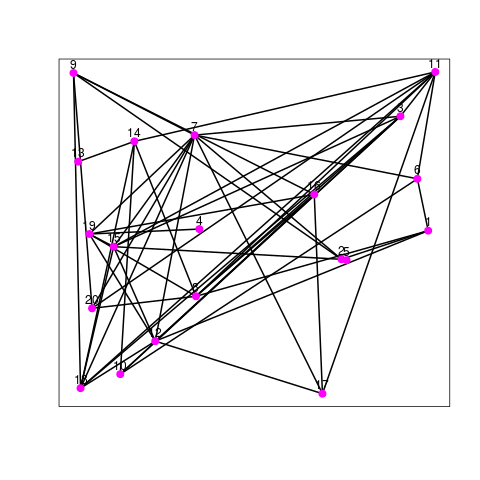
\includegraphics[width=.5\textwidth]{\fignet/FigCLADAG-LPM-X2}    
%         \onslide<7>
        $
        Y = \left( {\footnotesize
		\begin{array}{cccccc}
		0 & 1 & 1 & 0 & 1 & \dots \\
		0 & 0 & 1 & 0 & 1 & \dots \\
		0 & 0 & 0 & 0 & 0 & \dots \\
		0 & 0 & 0 & 0 & 1 & \dots \\
		0 & 0 & 0 & 0 & 0 & \dots \\
		\vdots & \vdots & \vdots & \vdots & \vdots & \ddots  
		\end{array}
        } \right)
        $ 
      \end{overprint}
    \end{tabular}
  \end{tabular}
  }

%====================================================================
\frame{\frametitle{A variety of state-space models}

  \paragraph{Latent position models.}
  \begin{itemize}
   \item \refer{HRH02}: 
   $$
   Z_i \in \Rbb^d, \qquad \logit\;\gamma(z, z') = a - |z-z'|
   $$
   \item \refer{HRT07}:
   $$
   Z_i \sim \sum_k p_k \Ncal_d(\mu_k, \sigma^2_k I)
   $$
%    \item \refer{LoS06}:
%    $$
%    Z_i \sim \Ucal_{[0, 1]}, \qquad \gamma(z, z'): [0, 1]^2 \rightarrow [0, 1] =: \text{graphon function}
%    $$
   \item \refer{DPV10}:
   $$
   Z_i \in \Scal_K, \qquad \gamma(z, z') = \sum_{k, \ell} z_k z'_\ell \gamma_{k\ell}
   $$
  \end{itemize} \pause
  
  In this talk, focus on
  \begin{itemize}
   \item the Stochastic Block Model (SBM) and
   \item the $W$-graph model (and its associated graphon).
  \end{itemize}

%   %\bigskip%\pause
%   \paragraph{Discrete.} Hidden class models. 
%   \begin{itemize}
%    \item \refer{NoS01}:
%    $$
%    Z_i \in \{1, \dots, K\}, \qquad \gamma(k, \ell) = \gamma_{k\ell}.   
%    $$
%   \end{itemize}
  }

%====================================================================
\frame{\frametitle{Stochastic Block Model (SBM)}

  \begin{tabular}{cc}
    \hspace{-.02\textwidth}
    \begin{tabular}{p{.5\textwidth}}
      \onslide+<1->{
	\paragraph{A mixture model for random graphs.}} \refer{NoS01}
      \onslide+<2->{
	\begin{itemize}
        \item Consider $n$ nodes ($i = 1..n$); \\ ~ } 
        \onslide+<3->{
        \item $Z_i = $ unobserved label of node $i$:
          $$
          \{Z_i\} \text{ iid } \sim \Mcal(1; \pi)
          $$
          $\pi = (\pi_1, ... \pi_K)$; \\ ~ } 
        \onslide+<4->{
        \item Edge $Y_{ij}$ depends on the labels:
          $\{Y_{ij}\}$ independent given $\{Z_i\}$,
          $$
          \Pr\{Y_{ij} = 1\} = \gamma(Z_i, Z_j)
          $$}
      \end{itemize}
    \end{tabular}
    & 
    \hspace{-.02\textwidth}
    \begin{tabular}{p{.5\textwidth}}
      \vspace{.02\textheight}
      \begin{overprint}
        \onslide<2>
        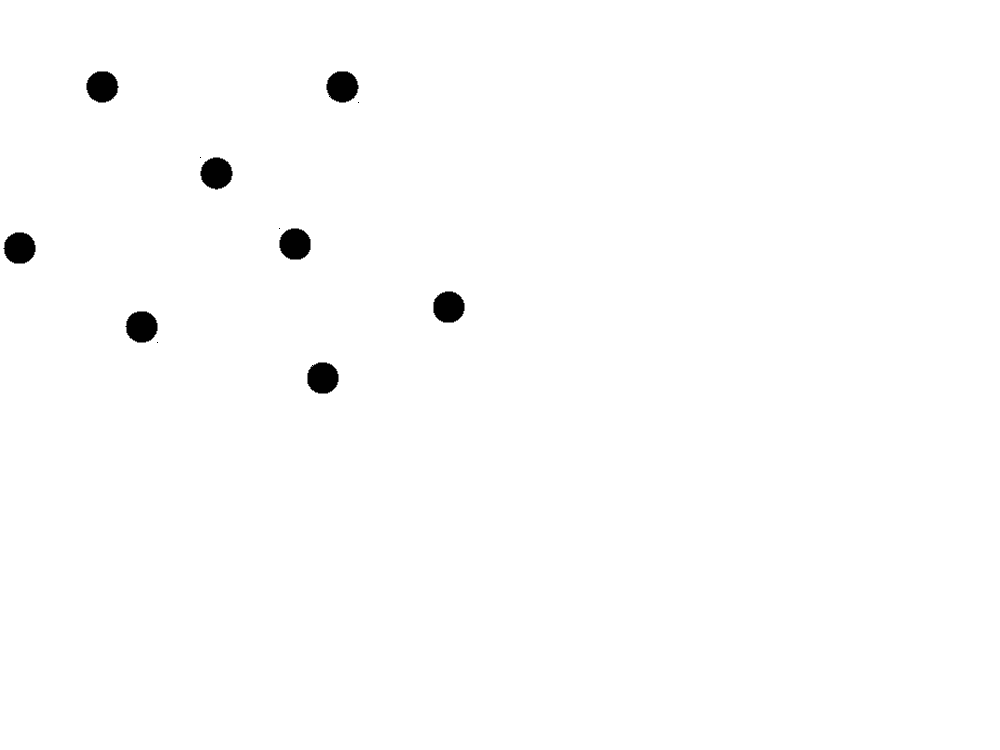
\includegraphics[width=.75\textwidth]{\fignet/FigSBM-Model-1}    
        \onslide<3>
        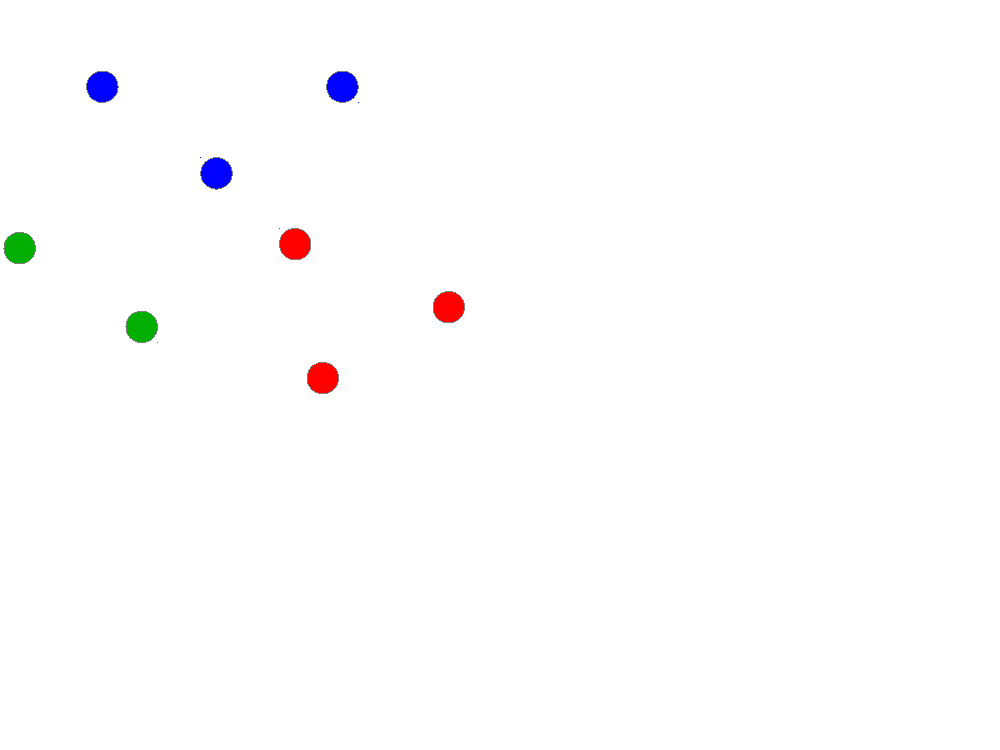
\includegraphics[width=.75\textwidth]{\fignet/FigSBM-Model-2}    
        \onslide<4>
        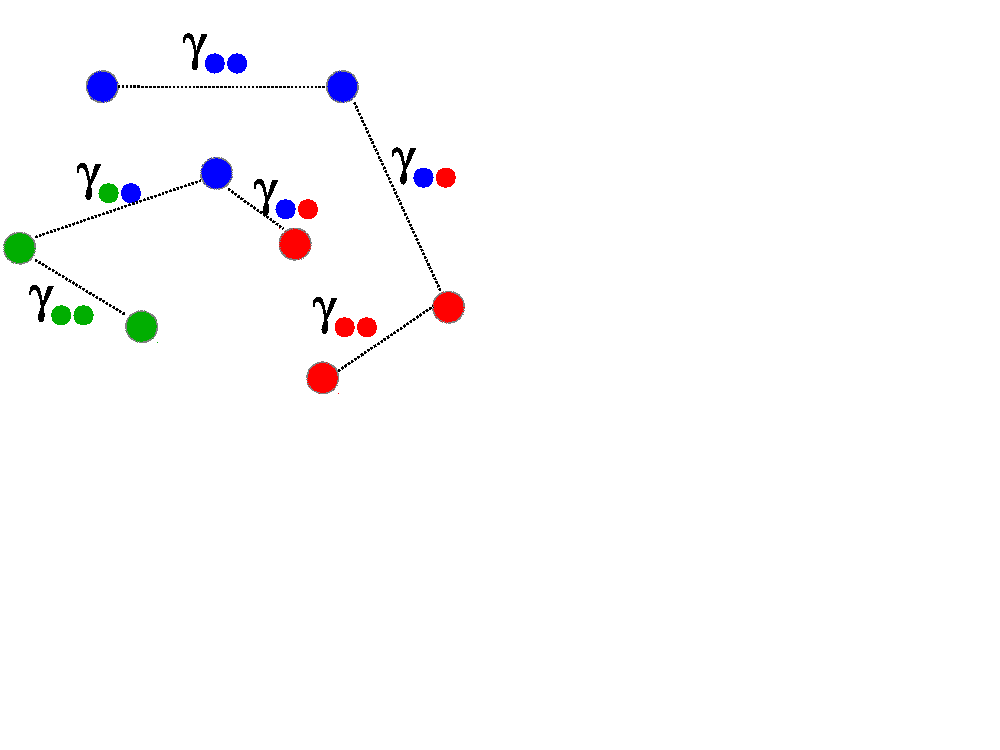
\includegraphics[width=.75\textwidth]{\fignet/FigSBM-Model-3}    
        \onslide<5>
        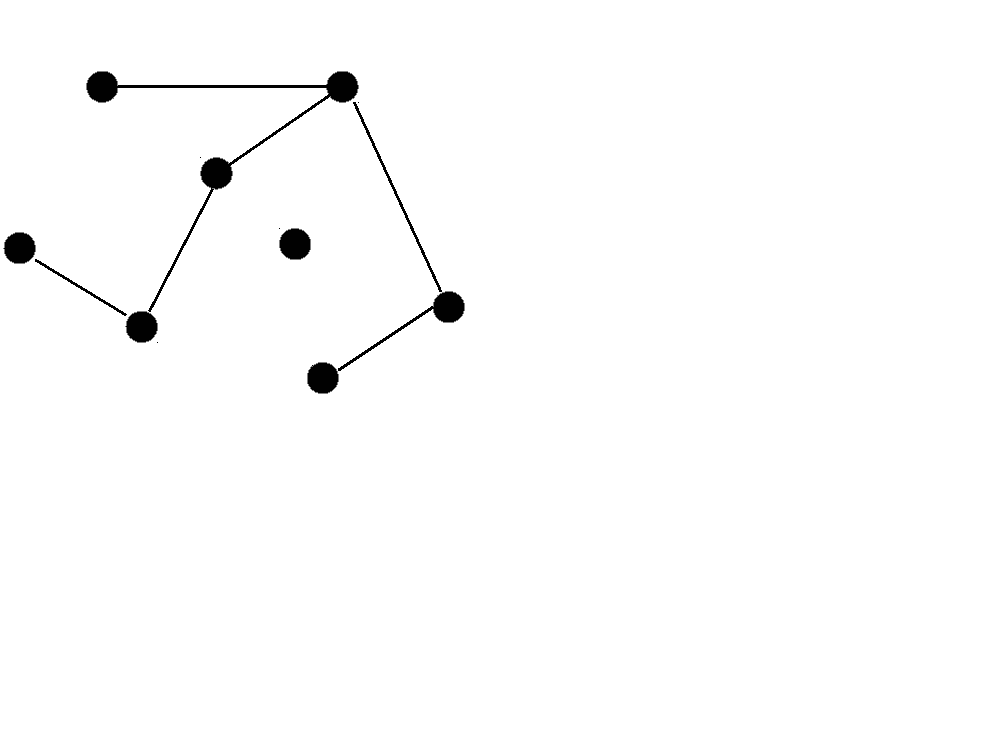
\includegraphics[width=.75\textwidth]{\fignet/FigSBM-Model-5}    
      \end{overprint}
    \end{tabular}
  \end{tabular}
  }

%====================================================================
\frame{ \frametitle{$W$-graph model}

  \begin{tabular}{cc}
    \hspace{-.02\textwidth}
    \begin{tabular}{p{.5\textwidth}}
	 Latent variables:
	 $$
	 (Z_i) \text{ iid } \sim \Ucal_{[0, 1]},
	 $$ ~\\
	 Graphon function $\gamma$:
	 $$
	 \gamma(z, z'): [0, 1]^2 \rightarrow [0, 1]
	 $$ ~\\    
	 Edges:
	 $$
	 \Pr\{Y_{ij} = 1\} = \gamma(Z_i, Z_j)
	 $$    
	 \end{tabular}
    & 
    \hspace{-.1\textwidth}
    \begin{tabular}{p{.5\textwidth}}
	 Graphon function $\gamma(z, z')$ \\
      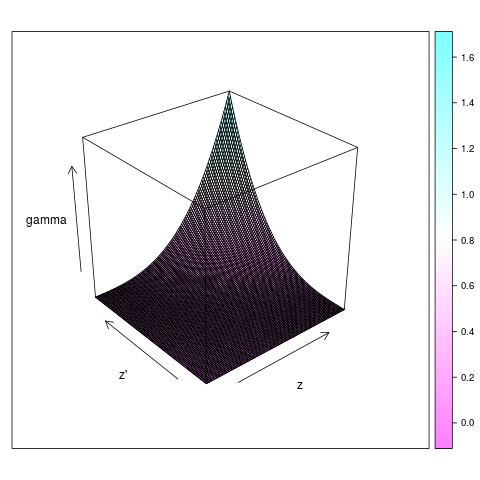
\includegraphics[width=.5\textwidth]{../FIGURES/FigCLADAG-W-graphon} \\
    \end{tabular}
  \end{tabular}
  
%   \medskip
%   \paragraph{Aim of this work:} provide an estimate of the graphon function.
%   Intensively studied in probability theory as a limit for dense graphs \refer{LoS06}.

 }

%====================================================================
\frame{\frametitle{Interpreting the graphon function}

  The graphon function provides a global picture of the network's topology.

  \bigskip \bigskip 
  \centerline{
  \begin{tabular}{ccc}
  'Scale free' & Community & Small world \\
  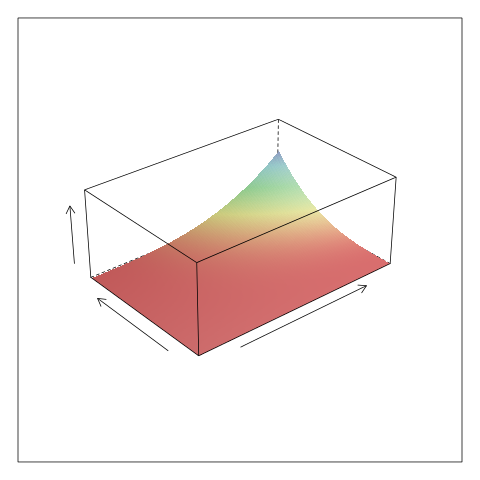
\includegraphics[width=.3\textwidth]{../FIGURES/EDD-ScaleFreeTrueGraphon} &
  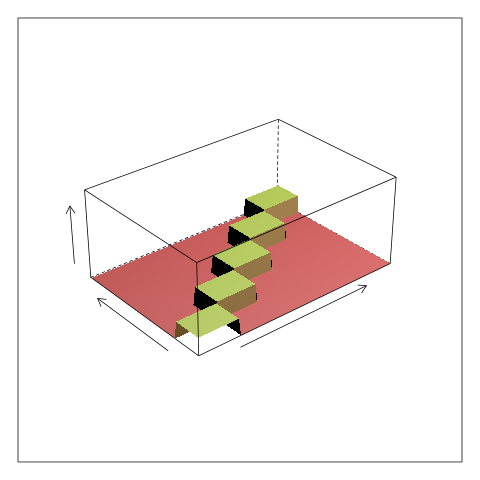
\includegraphics[width=.3\textwidth]{../FIGURES/CommunityTrueGraphon} &
  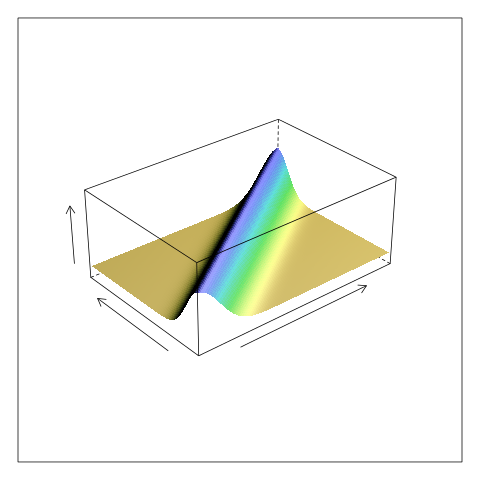
\includegraphics[width=.3\textwidth]{../FIGURES/SmallWorldTrueGraphon} 
  \end{tabular}
  } 
}

%====================================================================
\frame{ \frametitle{Few words about the $W$-graph}

  \paragraph{Probabilistic point of view.}
  \begin{itemize}
   \item $W$-graph have been mostly studied in the probability literature: \refer{LoS06}, \refer{DiJ08}
   \item Motif (sub-graph) frequencies are invariant characteristics of a $W$-graph.
   \item Intrinsic un-identifiability of the graphon function $\gamma$ is often overcome by imposing that $u \mapsto \int \gamma(u, v) \dd v$ is monotonous increasing.
  \end{itemize}

  \bigskip \bigskip \pause
  \paragraph{Statistical point of view.}
  \begin{itemize}
   \item Not much attention has been paid to its inference until recently: \refer{ACC13}, \refer{Cha14}, \refer{OlW14}, ...
   \item SBM can be used as a proxy for $W$-graph.
  \end{itemize}
}

%====================================================================
\subsection*{Some generalizations of latent space graph models}
%====================================================================
\frame{\frametitle{Some generalizations of latent space graph models}

  Latent space models can be extended in various directions. \pause

  \bigskip
  \paragraph{Weighted or directed networks.} Edges may have values: count, real, $\{0, +, -, \pm\}$, ... Latent space model can be adapted as
  $$
  Y_{ij} | Z_i, Z_j \sim \Fcal(\gamma(Z_i, Z_j))
  $$
  where $\Fcal$ is can be any distribution: Poisson, normal, multinomial, etc.
  
  \bigskip \bigskip \pause
  \paragraph{Accounting for covariates.} Latent space model can also accommodate for covariates, via a regression term:
  $$
  Y_{ij} | Z_i, Z_j \sim \Fcal(\gamma(Z_i, Z_j) + x'_{ij} \beta)
  $$
  where $x_{ij} = (x_{ij}^1, \dots x_{ij}^d)'$.
  
}

%====================================================================
%====================================================================
\section[Statistical inference of latent space models]{Statistical inference of latent space models (focus on SBM)}
%====================================================================
\frame{\frametitle{Statistical inference of latent space models}}

%====================================================================
\subsection*{Incomplete data models}
%====================================================================
\frame{\frametitle{Incomplete data models}

	\paragraph{Aim.} Based on the observed network $Y = (Y_{ij})$, one want typically to infer
	\begin{itemize}
	\item the parameters
	$$
	\theta = (\pi, \gamma)
	$$
	\item the hidden states 
	$$
	Z = (Z_i)
	$$
	\end{itemize}

	\bigskip \bigskip \pause
	State space models belong to the class of incomplete data models as
	\begin{itemize}
	\item the edges $(Y_{ij})$ are observed,
	\item the latent positions (or status) $(Z_i)$ are not, 
	\item and neither are the parameter.
	\end{itemize}
}

%====================================================================
\frame{\frametitle{Frequentist or Bayesian inference}

  \paragraph{Frequentist inference.} $\theta$ is fixed and $Z$ is random. The aim is then to
  \begin{itemize}
   \item provide an estimate $\widehat{\theta}$ of $\theta$,
   \item provide the conditional distribution $P_\theta(Z|Y)$ (for classification purposes and as a side product of the inference).
  \end{itemize}
  
  \bigskip \bigskip \pause
  \paragraph{Bayesian inference.} Both $\theta$ and $Z$ are random. The aim is then to
  \begin{itemize}
   \item provide the joint conditional distribution $P(\theta, Z | Y)$.
  \end{itemize}
    
  \bigskip \bigskip \pause
  Whatever the approach, we have to deal with conditional distributions:
  $$
  P_\theta(Z|Y) \qquad \text{or} \qquad P(\theta, Z | Y).
  $$
}

%====================================================================
\frame{\frametitle{Conditional distributions (1/2)}

  \begin{tabular}{cc}
    \hspace{-.02\textwidth}
    \begin{tabular}{p{.5\textwidth}}
      \onslide+<1->{
        \paragraph{Graphical models} describe the conditional independences between the random variables from a model \refer{Lau96}. \\ ~\\ }
        \onslide+<2->{\paragraph{Frequentist setting:}}
        \begin{itemize}
        \onslide+<2->{\item iid $Z_i$'s,}
        \onslide+<3->{\item $P(Y_{ij} | Z_i, Z_j)$,}
        \onslide+<4->{\item $P(Z_i, Z_j|Y)$: graph moralization,}
        \onslide+<5->{\item this holds for each pair $(i, j)$,}
        \end{itemize}
    \end{tabular}
    & 
    \hspace{-.02\textwidth}
    \begin{tabular}{p{.5\textwidth}}
	 \begin{overprint}
        \onslide<2>
        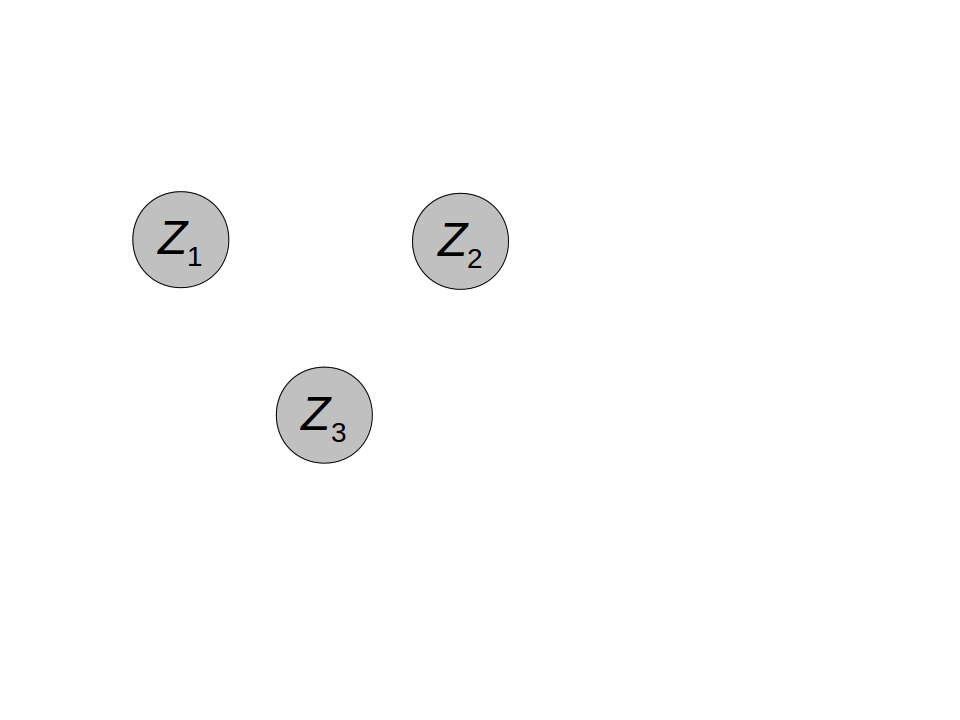
\includegraphics[width=0.6\textwidth]{../FIGURES/FigSBM-Z}
%        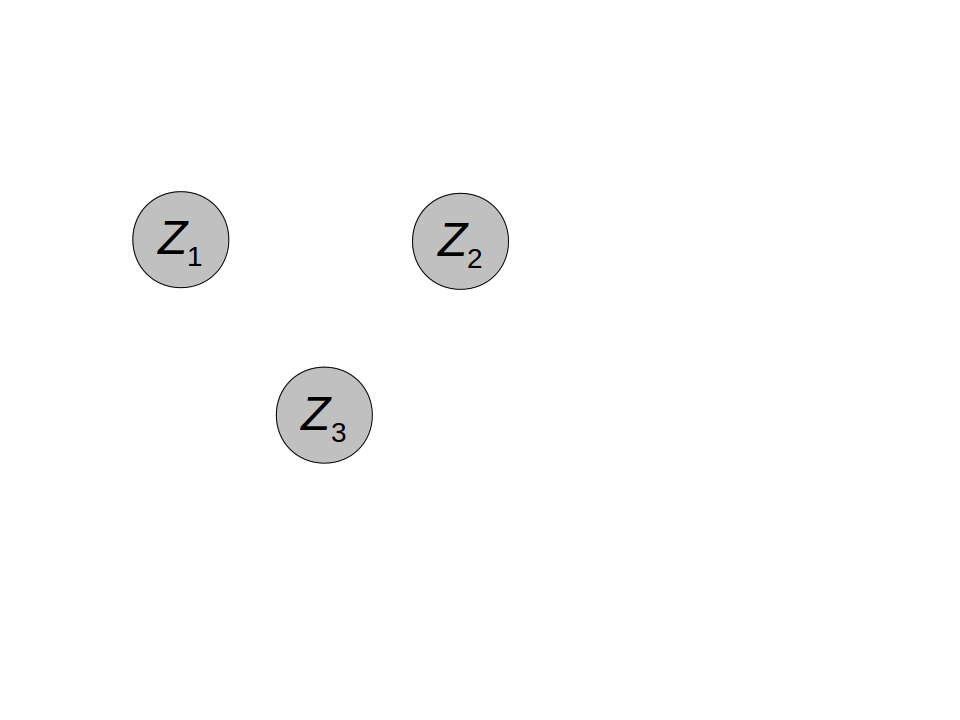
\epsfig{file=../FIGURES/FigSBM-Z.eps, clip=, width=0.6\textwidth}
        \onslide<3>
        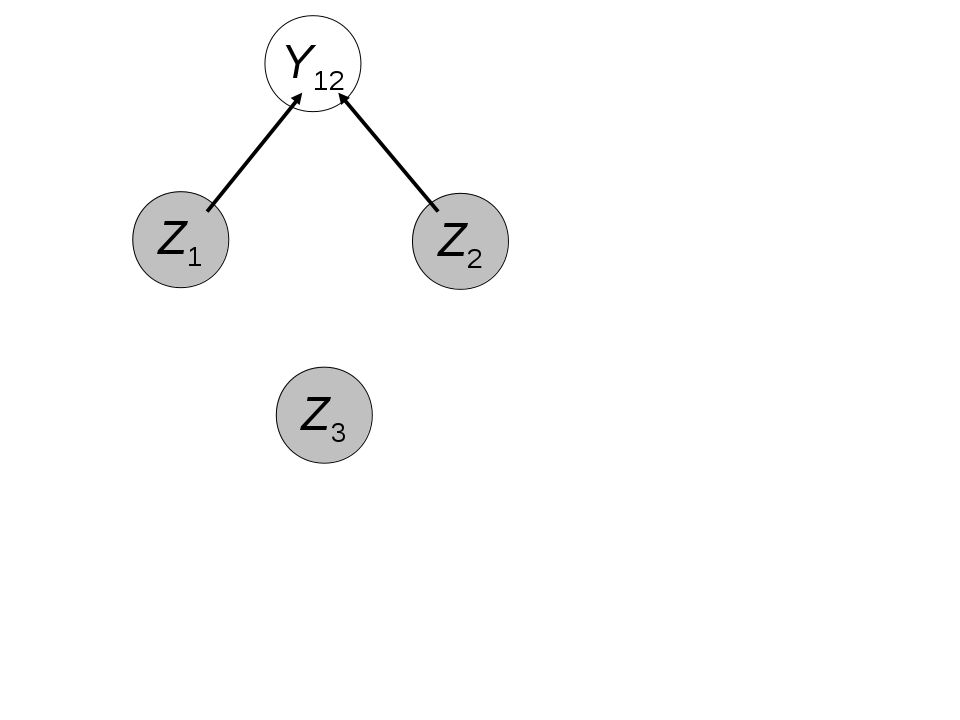
\includegraphics[width=0.6\textwidth]{../FIGURES/FigSBM-Z-Y12}
%         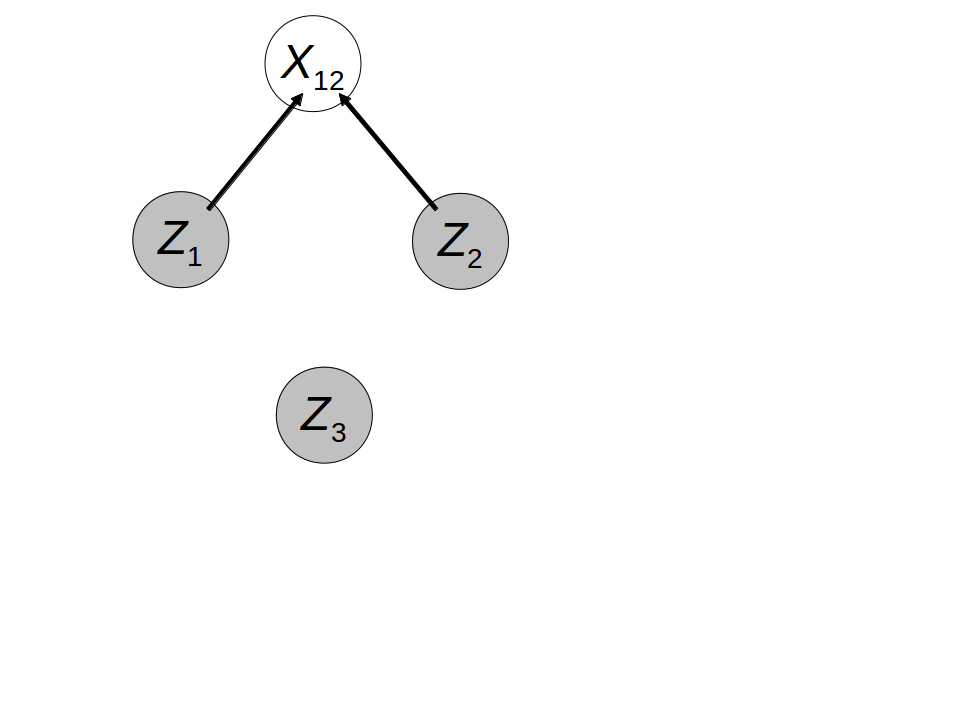
\epsfig{file=../FIGURES/FigSBM-Z-X12.eps, clip=, width=0.6\textwidth}
        \onslide<4>
        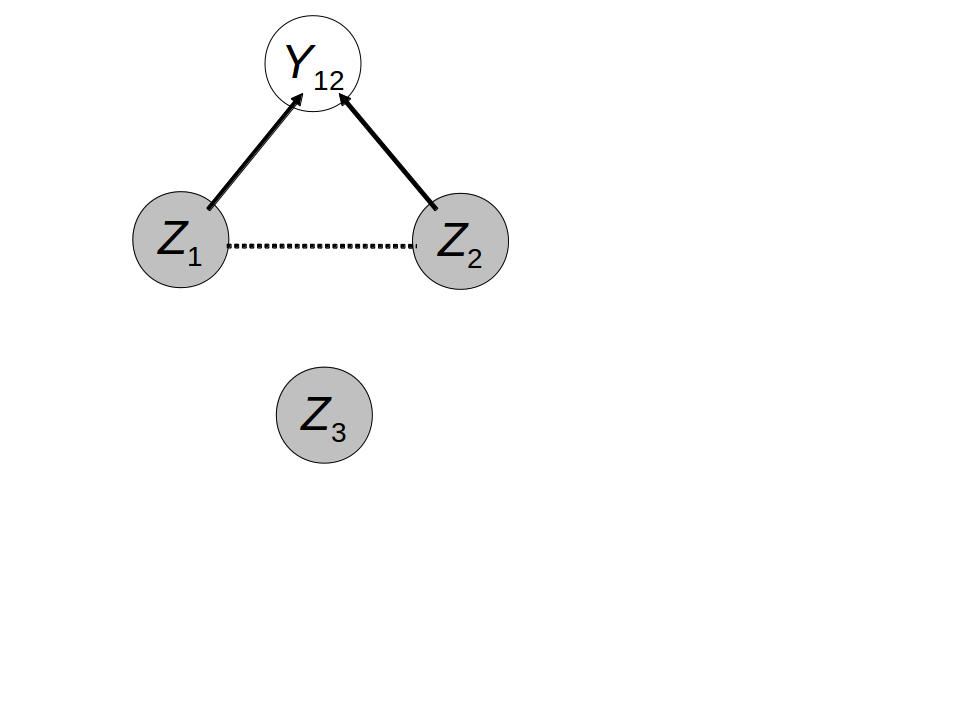
\includegraphics[width=0.6\textwidth]{../FIGURES/FigSBM-Z-Y12-Moral} 
%         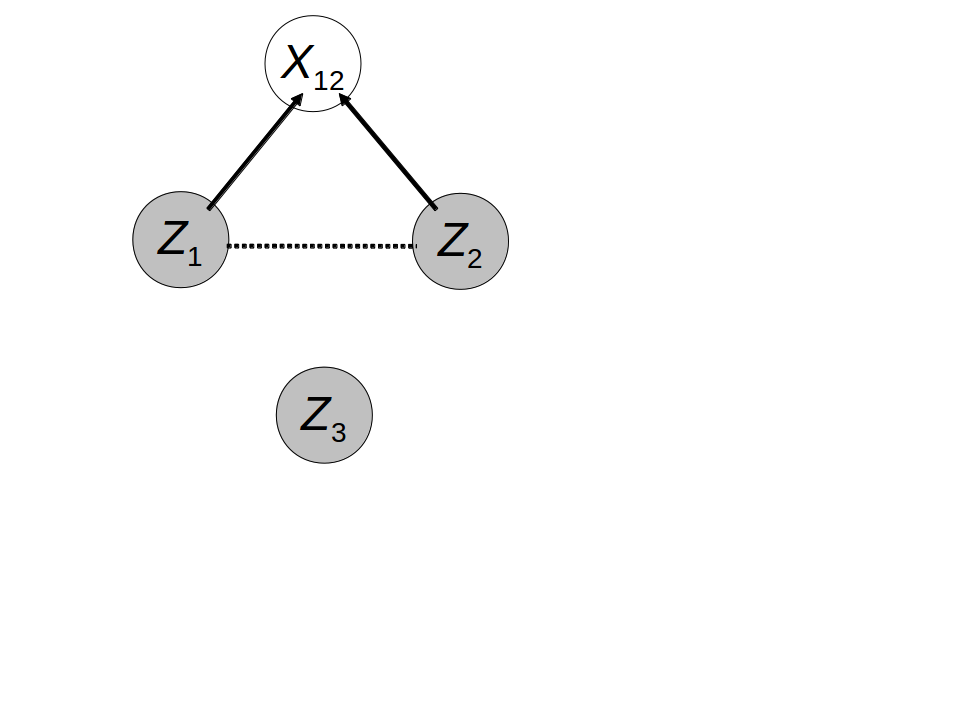
\epsfig{file=../FIGURES/FigSBM-Z-X12-Moral.eps, clip=, width=0.6\textwidth} 
        \onslide<5>
        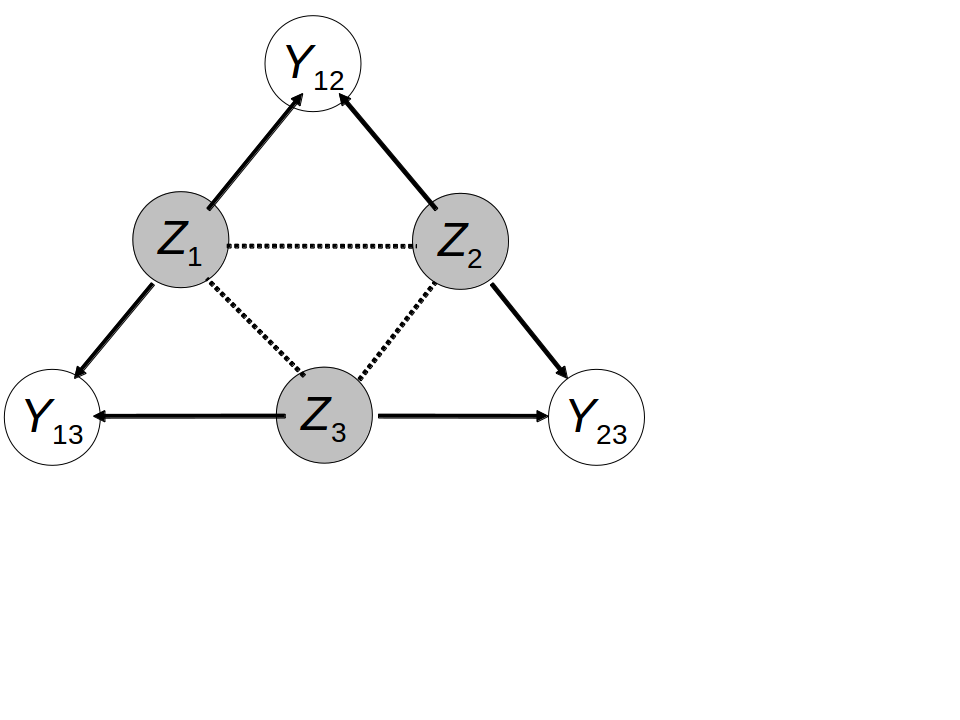
\includegraphics[width=0.6\textwidth]{../FIGURES/FigSBM-Z-Y-Moral} 
%         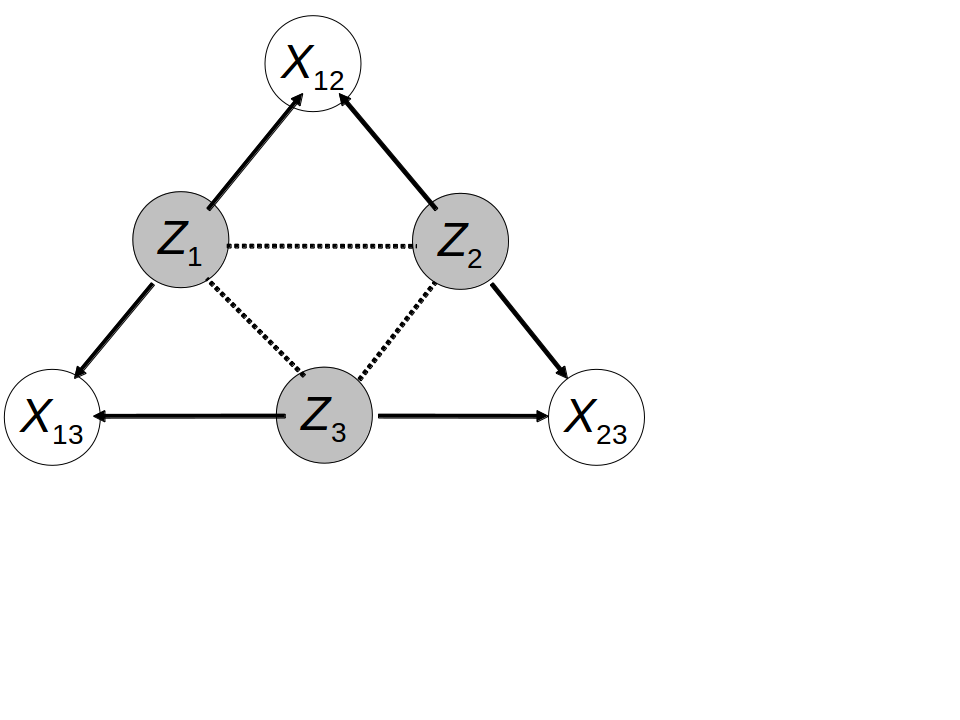
\epsfig{file=../FIGURES/FigSBM-Z-X-Moral.eps, clip=, width=0.6\textwidth} 
        \onslide<6->
        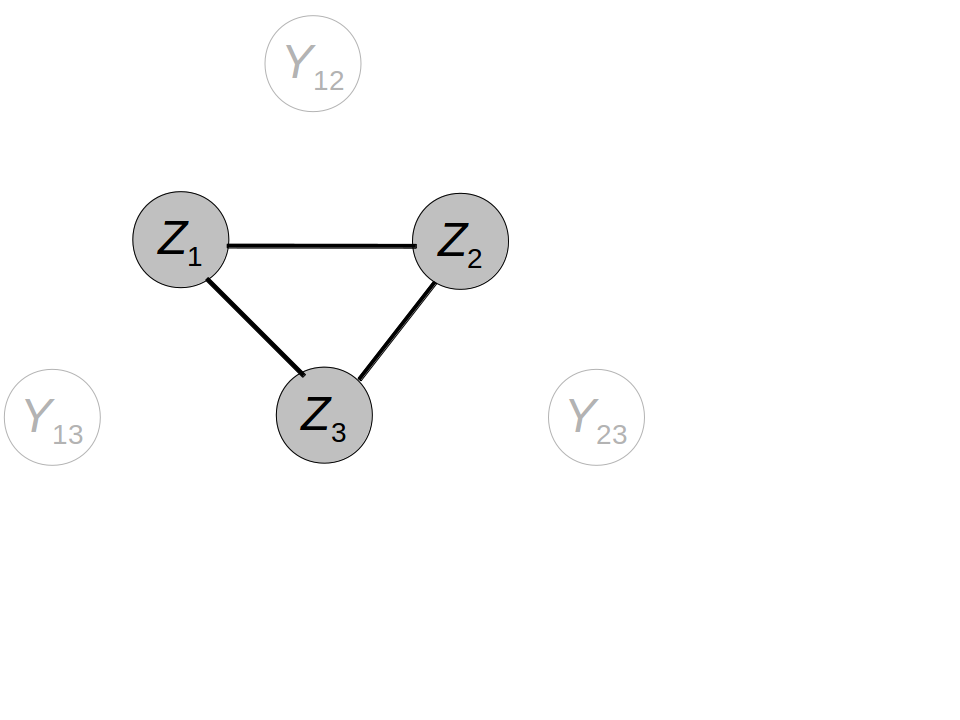
\includegraphics[width=0.6\textwidth]{../FIGURES/FigSBM-ZcondY}
%         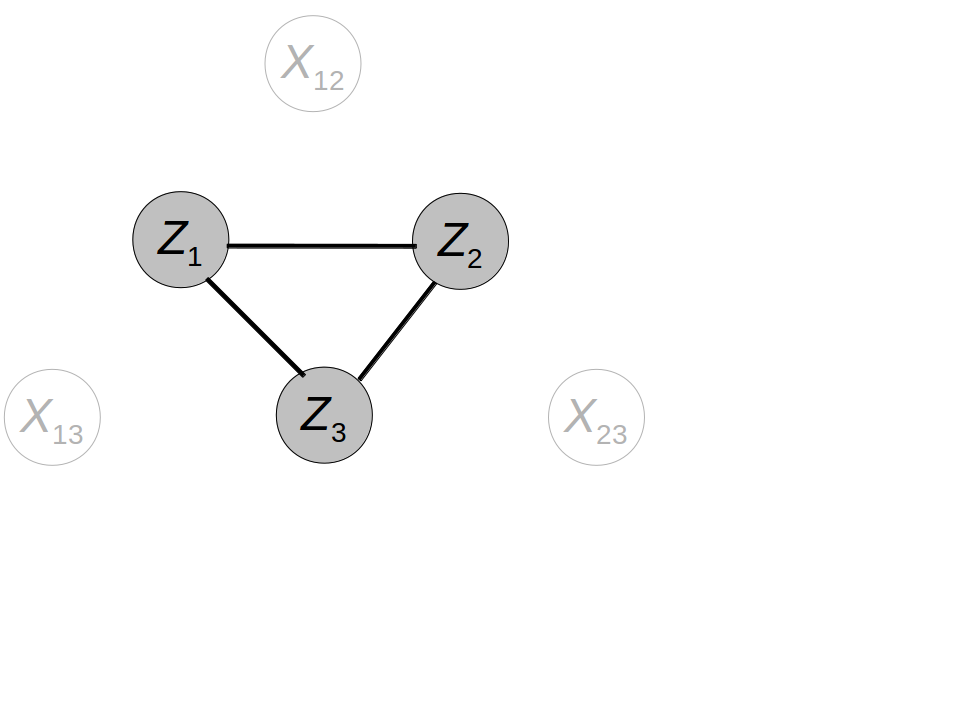
\epsfig{file=../FIGURES/FigSBM-ZcondX.eps, clip=, width=0.6\textwidth}
      \end{overprint}
    \end{tabular}
  \end{tabular}

  \onslide+<6->{
%     \vspace{-1.5cm}
    \paragraph{Conditional distribution.} The dependency graph of
    $Z$ given $Y$ is a clique. \\
    \ra No factorization can be hoped (unlike for HMM). \\
    \ra $P_\theta(Z | Y)$ can not be computed
    (efficiently). \\
%     \ra Variational techniques may help as they provide 
%     $$
%     \Pt(Z) \simeq P(Z | Y).
%     $$
  }
}

%====================================================================
\frame{\frametitle{Conditional distributions (2/2)}

  \vspace{-.07\textheight}
  \begin{tabular}{cc}
    \hspace{-.02\textwidth}
    \begin{tabular}{p{.4\textwidth}}  
	 \paragraph{Bayesian perspective.} Things get worst because $\theta = (\pi, \gamma)$ is also random. 
	 
	 \bigskip
	 \paragraph{Model:}
      \begin{itemize}
      \onslide+<2->{\item $P(\theta)$}
      \onslide+<3->{\item $P(Z|\pi)$}
      \onslide+<4->{\item $P(Y|\gamma, Z)$}
      \onslide+<5->{\item $P(\theta, Z |Y)$ is even more involved}.
      \end{itemize}
      \vfill
    \end{tabular}
    & 
    %\hspace{-.02\textwidth}
    \begin{tabular}{p{.6\textwidth}}
	 \vspace{1.3cm}
	 \begin{overprint}
	 \onslide<2>
	 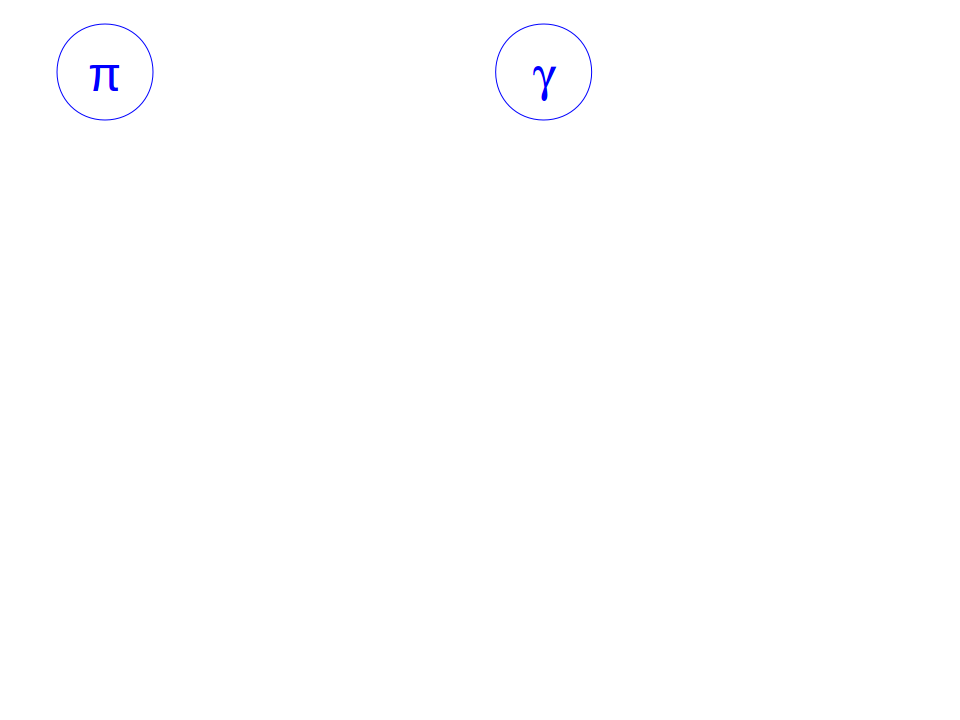
\includegraphics[width=.6\textwidth]{\fignet/FigSBM-Bayes-pi-gamma}    
	 \onslide<3>
	 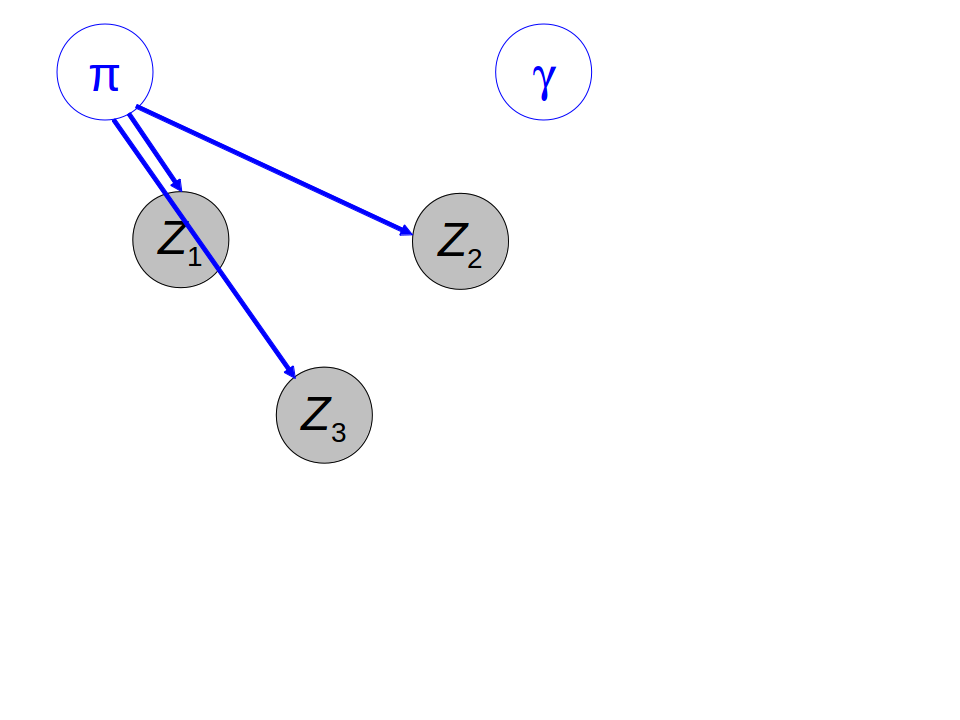
\includegraphics[width=.6\textwidth]{\fignet/FigSBM-Bayes-pi-gamma-Z}    
	 \onslide<4>
	 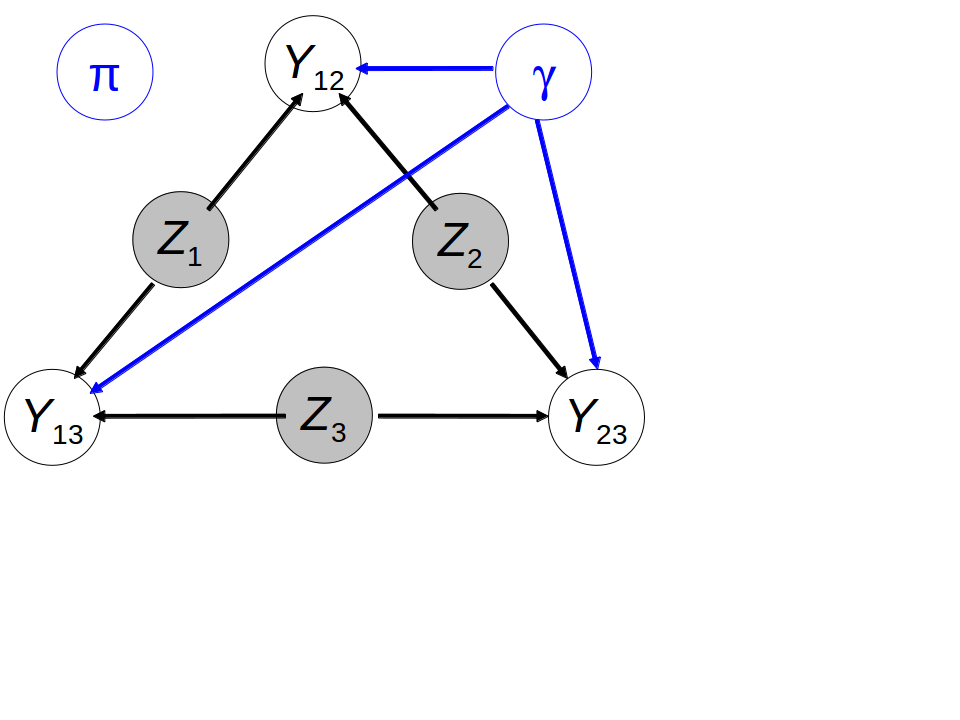
\includegraphics[width=.6\textwidth]{\fignet/FigSBM-Bayes-gamma-Z-Y}    
	 \onslide<5->
	 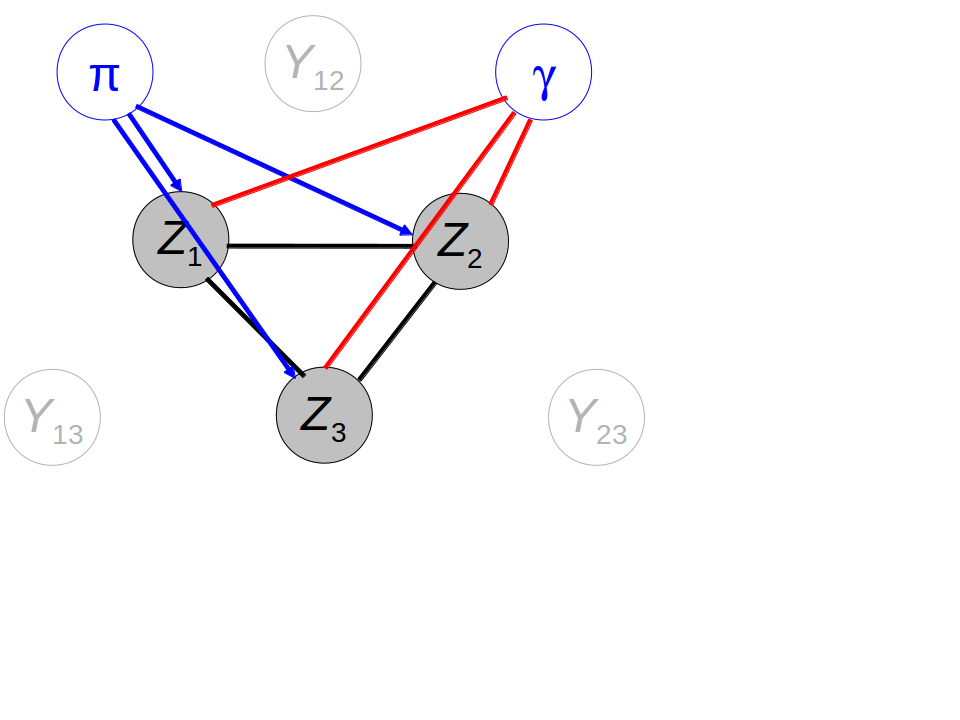
\includegraphics[width=.6\textwidth]{\fignet/FigSBM-Bayes-theta-ZcondY}    
	 \end{overprint}
	 \vfill
    \end{tabular}
  \end{tabular}
  
  \vspace{-.1\textheight}
  \onslide+<6->{Both frequentist and Bayesian inference require the calculation of conditional distributions that can not be computed. \\
  \ra Either sampling (MCMC) or approximation is required.}

}

%====================================================================
\subsection*{Variational (Bayes) inference}
%====================================================================
\frame{\frametitle{Variational (Bayes) inference}

  \paragraph{Variational approximations} aim at replacing an intractable exact distribution $P$ with a tractable approximate distribution $\Pt$. Typically:
  \begin{eqnarray*}
   P_\theta(Z|Y) & \approx & \prod_i \Pt_{\theta, Y}(Z_i) \\
   P(\theta, Z|Y) & \approx & \Pt_Y(\theta) \times \Pt_Y(Z) \\
   P(\theta, Z|Y) & \approx & \Pt_Y(\theta) \times \prod_i \Pt_{Y}(Z_i)\\
  \end{eqnarray*}
  
  \paragraph{Popular strategy:} minimize the K�llback-Leibler divergence between $\Pt$ and $P$:
  $$
  \min KL[\Pt(Z) || P_\theta(Z|Y)]
  \qquad \text{or} \qquad
  \min KL[\Pt(\theta, Z) || P(\theta, Z|Y)]
  $$
  
  \bigskip
  \ra Variational EM (VEM) algorithm \refer{WaJ08}. \\
  \ra Variational Bayes EM (VBEM) algorithm \refer{BeG03}.
}

%====================================================================
\frame{\frametitle{VBEM inference for SBM: {\sl E. coli}'s operon network}

  \vspace{-0.5cm}
  \hspace{-0.5cm}
  \begin{tabular}{cc}         
    \begin{tabular}{p{0.45\textwidth}}
%     \begin{overprint}
       \onslide<1->{
       \vspace{-1cm}
       \includegraphics[width=.45\textwidth]{\fignet/im_EcoliVEM_2} \\
       %~\\
       \refer{PMD09}
       }
%     \end{overprint}
    \end{tabular}
    &
    \begin{tabular}{p{0.45\textwidth}}
     \onslide+<2->{
      \vspace{-.3cm}
      \paragraph{Meta-graph representation.} \\
      %\vspace{-.02\textwidth}
      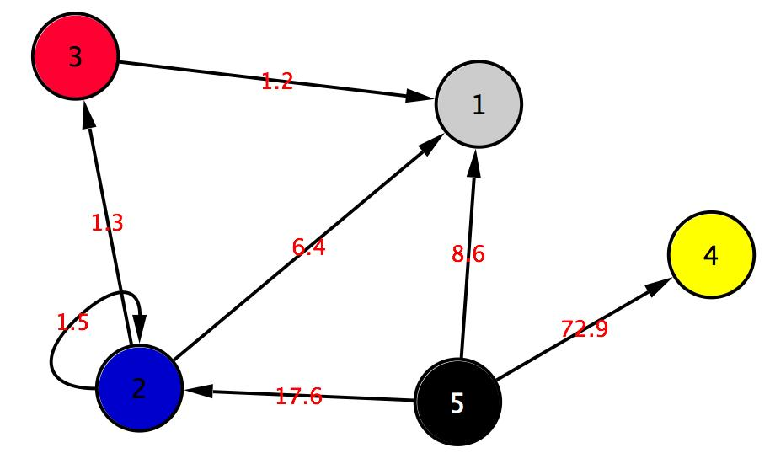
\includegraphics[width=.35\textwidth]{\fignet/VEMmetagraphe}  \\
     }
     \onslide+<3->{
      \vspace{-.3cm}
      \paragraph{Parameter estimates.} $K = 5$     \\
      \includegraphics[width=.35\textwidth]{../FIGURES/im-pi1BVEM}\\        
      \includegraphics[width=.35\textwidth]{../FIGURES/im-pi2BVEM}\\
      \includegraphics[width=.35\textwidth]{../FIGURES/im-pi3BVEM}\\
      \includegraphics[width=.35\textwidth]{../FIGURES/im-pi4BVEM}\\
      \includegraphics[width=.35\textwidth]{../FIGURES/im-pi5BVEM}\\
      \hline 
      \includegraphics[width=.35\textwidth]{../FIGURES/im-alphaBVEM}\\
     }
    \end{tabular}
  \end{tabular}
  }

%====================================================================
\frame{ \frametitle{Accuracy of {\VBEM} estimates for SBM: Simulation study}

  \paragraph{Credibility intervals:}   $\pi_1$: $+$,
  $\gamma_{11}$: \textcolor{red}{$\triangle$}, $\gamma_{12}$:
  \textcolor{blue}{$\circ$}, $\gamma_{22}$: \textcolor{green}{$\bullet$} 
  $$
  \includegraphics[width=1\textwidth]{../FIGURES/im-ICQ2-2-new} 
  $$
  \pause
  \emphase{Width of the posterior credibility intervals.}
  {$\pi_1$}, \textcolor{red}{$\gamma_{11}$},
  \textcolor{blue}{$\gamma_{12}$}, \textcolor{green}{$\gamma_{22}$}
  \\
  \includegraphics[width=1\textwidth]{../FIGURES/im-ICQ2-3} \\
   \refer{GDR11}

 }
 

%====================================================================
\frame{\frametitle{First half summary}

  \begin{itemize}
   \item Latent space graph models are useful to describe network heterogeneity.
   \item Their statistical inference raises some specific issues.
   \item Variational approximations help to circumvent these issues.
  \end{itemize}

  \bigskip \pause
  And also
  \begin{itemize}
   \item Theoretical justifications of these approximations exist for SBM: \refer{CDP12}, \refer{MaM14}
   \item VEM and VBEM algorithms have been specifically developed for SBM: \refer{DPR08}, \refer{LBA11b}
   \item Model selection (choice of $K$ has also be addressed): \Refer{same refs as above}.
  \end{itemize}


}


%====================================================================
%====================================================================
\section{From SBM to $W$-graph: Averaging models}
%====================================================================
\frame{\frametitle{From SBM to $W$-graph: Averaging models}}

%====================================================================
\subsection*{SBM as a $W$-graph model}
%====================================================================
%====================================================================
\frame{ \frametitle{SBM as a $W$-graph model}

  \begin{tabular}{cc}
    \hspace{-.02\textwidth}
    \begin{tabular}{p{.5\textwidth}}
	 Latent variables:
	 $$
	 (Z_i) \text{ iid } \sim \Mcal(1, \pi)
	 $$ ~\\
	 Blockwise constant graphon:
	 $$
	 \gamma(z, z') = \gamma_{k\ell}
	 $$ ~\\
	 Edges:
	 $$
	 \Pr\{Y_{ij} = 1\} = \gamma(Z_i, Z_j)
	 $$    
	 \end{tabular}
    & 
    \hspace{-.1\textwidth}
    \begin{tabular}{p{.5\textwidth}}
	 Graphon function $\gamma^{SBM}_K(z, z')$ \\
      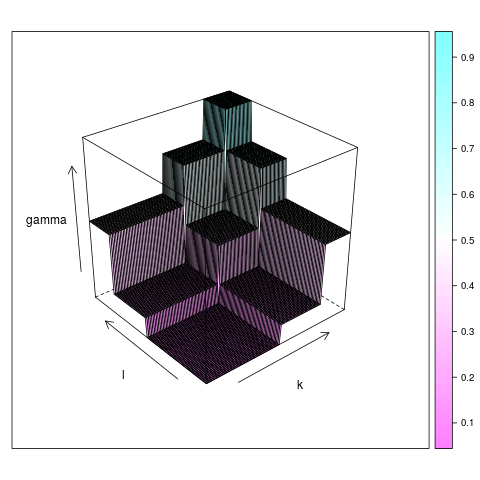
\includegraphics[width=.5\textwidth]{../FIGURES/FigCLADAG-SBM-graphon} \\
    \end{tabular}
  \end{tabular}

  \ra block widths $= \pi_k$, block heights $\gamma_{k\ell}$
 }

%====================================================================
\frame{ \frametitle{Variational Bayes estimation of $\gamma(z, z')$}

%   \paragraph{General idea.} Estimate the true $\gamma$ with a blockwise constant function $\gamma_K^{SBM}$ with $K$ classes.

  \begin{tabular}{cc}
    \hspace{-.02\textwidth}
    \begin{tabular}{p{.45\textwidth}}
    \paragraph{VBEM inference} provides the \\approximate posteriors:
    \begin{eqnarray*}
    (\pi | Y) & \approx & \text{Dir}(\pi^*) \\
    (\gamma_{k\ell} | Y) & \approx & \text{Beta}(\gamma^{0*}_{k\ell}, \gamma^{1*}_{k\ell}) 
    \end{eqnarray*}
    ~
    
    \bigskip 
    \paragraph{Estimate of $\gamma(u, v)$.} 
    Due \\
    to the uncertainty of the $\pi_k$, \\
    the posterior mean of $\gamma^{SBM}_K$  \\
    is smooth
    
    \bigskip 
    (Explicit integration using \refer{GoS10})
%     $$
%     \widehat{\gamma}_K^{SBM}(u, v) = \widetilde{\Esp}\left(\gamma_{C(u), C(v)} | Y\right)
%     $$
%     where $C(u) = 1 + \sum_k \Ibb\{\sigma_k \leq u\}$. \\ ~
%     \\
%     \refer{GoS10}
    \end{tabular}
    & 
    \hspace{-.05\textwidth}
    \begin{tabular}{p{.5\textwidth}}
	 Posterior mean $\widetilde{\Esp}(\gamma^{SBM}_K(z, z') | Y, K)$ \\
      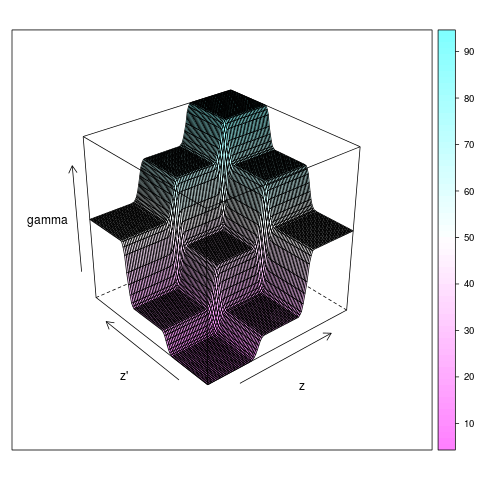
\includegraphics[width=.5\textwidth]{../FIGURES/FigGraphon-SBM-average} \\
% 	 Posterior mean of $\gamma^{SBM}_K(z, z')$ \\
%     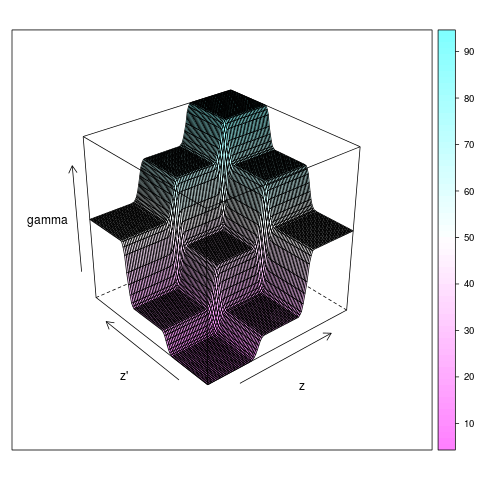
\includegraphics[width=.6\textwidth]{../FIGURES/FigGraphon-SBM-average} \\
    \end{tabular}
  \end{tabular}
  
}

%====================================================================
\subsection*{Bayesian model averaging}
%====================================================================
\frame{\frametitle{Bayesian model averaging}

%   There is no 'true' $K$ when inferring the graphon of a $W$ graph.
  
%   \bigskip
  \paragraph{Bayesian model averaging (BMA).} Consider a series of models $1, \dots, K, \dots$ in which a certain function of the parameter $f(\theta)$ can always be defined.
  
  \bigskip
  \begin{itemize}
   \item \pause Bayesian inference within each model $K$ provides the posterior
   $$
   P(\theta|K, Y) \qquad \rightarrow \qquad P(f(\theta) | K, Y).
   $$ ~\\
   \item \pause BMA \refer{HMR99} relies on the marginal posterior of $f(\theta)$:
   $$
   P(f(\theta) | Y) = \sum_K P(K | Y) P(f(\theta) | K, Y).
   $$
  \end{itemize}

}

%====================================================================
\frame{\frametitle{Variational Bayes model averaging}

  \paragraph{Pushing it further:} Consider the model $K$ as an additional hidden variable:
  \begin{eqnarray*}
  P(Z, \theta, K|Y) & \approx & \Pt(Z, \theta, K) \\
  & := & \Pt(Z|K) \times \Pt(\theta|K) \times \Pt(K)  \end{eqnarray*}
  Note that no additional independence assumption is needed.
  
  \bigskip \bigskip \pause
  \paragraph{Variational Bayes model averaging (VBMA).} The optimal\footnote{in terms of K�llback-Leibler divergence} approximation of $P(K|Y)$ satisfies \refer{VMR12}: 
  $$
    \Pt(K) \propto P(K) e^{\log P(Y|K) - KL(K)} = P(K|Y) e^{-\emphase{KL(K)}}
  $$ ~ \\
  where $KL(K) = KL[\Pt(Z, \theta|K); P(Z,  \theta|Y, K)]$. 

}

%====================================================================
\subsection*{Inferring the graphon function}
%====================================================================
\frame{\frametitle{Inferring the graphon function}

  \paragraph{Model averaging:} There is no 'true $K$' in the $W$-graph model.

  \bigskip \bigskip
  \paragraph{Apply VBMA recipe to $\gamma(z, z')$.}
  For $K = 1 .. K_{\max}$, fit an SBM model via VBEM and compute
  $$
  \widehat{\gamma}_K^{SBM}(z, z') = \widetilde{\Esp}[\gamma_{C(z), C(z')} | Y, K].
  $$
  
  \pause \bigskip \bigskip
  Then perform model averaging as
  $$
  \widehat{\gamma}(z, z') = \widetilde{\Esp}[\gamma_{C(z), C(z')} | Y] = \sum_K \Pt(K) \widehat{\gamma}_K^{SBM}(z, z'),
  $$
  \Refer{Latouche and R. (2013)}\nocite{LaR13}.
%   \end{itemize}
}

%====================================================================
\frame{\frametitle{PPI network}

  Like many PPI networks, {\sl E. coli}'s network is highly concentrated around few nodes.

  \begin{tabular}{cc}
    \begin{tabular}{p{.5\textwidth}}
	 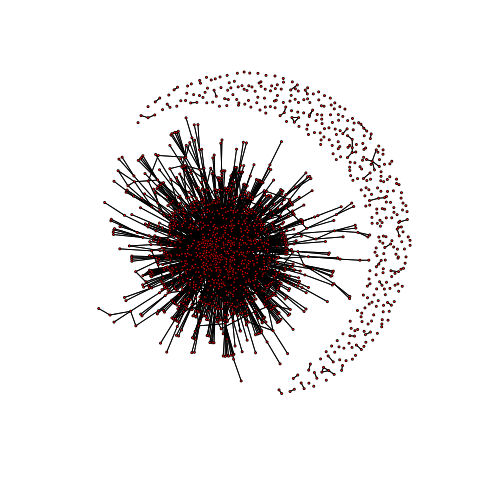
\includegraphics[width=.45\textwidth]{../FIGURES/Ecoli20060402-graph}
    \end{tabular}
    & 
    \hspace{-.1\textwidth}
    \begin{tabular}{p{.5\textwidth}}
	 \begin{overprint}
	 \onslide<1>
	 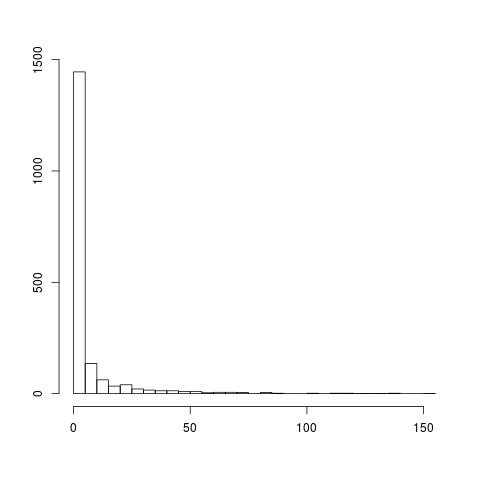
\includegraphics[width=.45\textwidth]{../FIGURES/Ecoli20060402-degree}
	 \onslide<2>
	 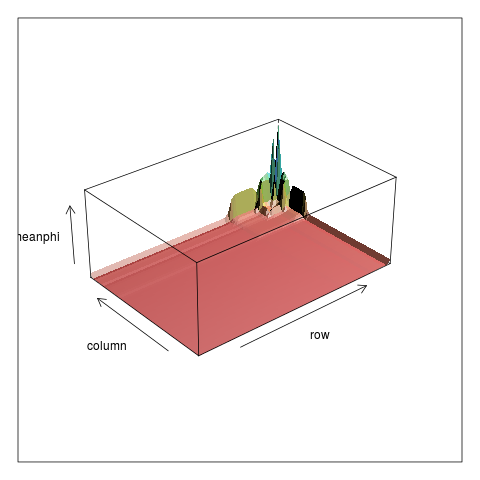
\includegraphics[width=.45\textwidth]{../FIGURES/Ecoli20060402-graphon}
	 \end{overprint}
    \end{tabular}
  \end{tabular}
}

%====================================================================
\frame{\frametitle{Ecological network between fungal species}

  Link between 2 fungi if they are observed on one common host.

  \begin{tabular}{cc}
    \begin{tabular}{p{.5\textwidth}}
	 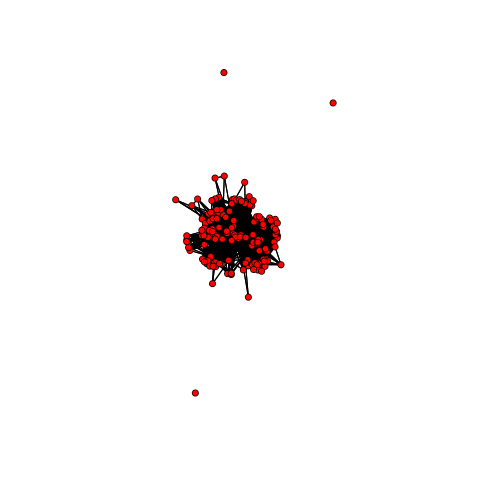
\includegraphics[width=.45\textwidth]{../FIGURES/Fungi-graph}
    \end{tabular}
    & 
    \hspace{-.1\textwidth}
    \begin{tabular}{p{.5\textwidth}}
	 \begin{overprint}
	 \onslide<1>
	 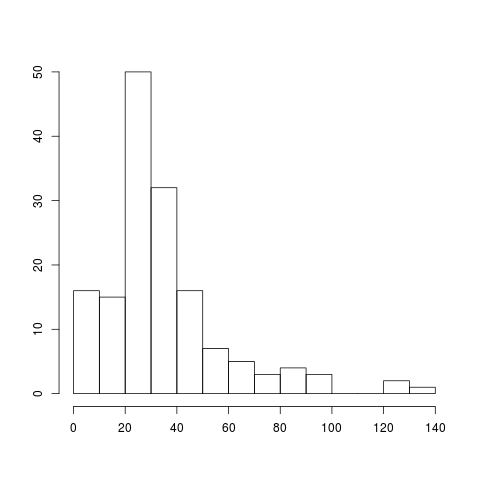
\includegraphics[width=.45\textwidth]{../FIGURES/Fungi-degree}
	 \onslide<2>
	 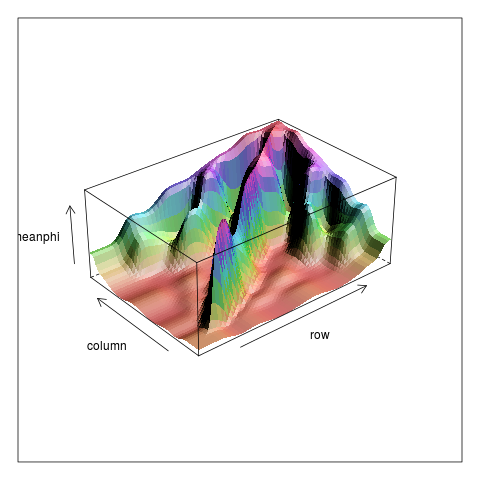
\includegraphics[width=.45\textwidth]{../FIGURES/Fungi-graphon}
	 \end{overprint}
    \end{tabular}
  \end{tabular}
}

%====================================================================
\frame{\frametitle{Brain network}

  Links = connexions between areas of the macaque's cortex

  \begin{tabular}{cc}
    \begin{tabular}{p{.5\textwidth}}
	 \includegraphics[width=.45\textwidth]{../FIGURES/Macaque-graph}
    \end{tabular}
    & 
    \hspace{-.1\textwidth}
    \begin{tabular}{p{.5\textwidth}}
	 \begin{overprint}
	 \onslide<1>
	 \includegraphics[width=.45\textwidth]{../FIGURES/Macaque-degree}
	 \onslide<2>
	 \includegraphics[width=.45\textwidth]{../FIGURES/Macaque-graphon}
	 \end{overprint}
    \end{tabular}
  \end{tabular}
}

%====================================================================
\frame{\frametitle{Blog network (non-biological)}

  Links = connexions between French political blogs

  \begin{tabular}{cc}
    \begin{tabular}{p{.5\textwidth}}
	 \includegraphics[width=.45\textwidth]{../FIGURES/Blog-graph}
    \end{tabular}
    & 
    \hspace{-.1\textwidth}
    \begin{tabular}{p{.5\textwidth}}
	 \begin{overprint}
	 \onslide<1>
	 \includegraphics[width=.45\textwidth]{../FIGURES/Blog-degree}
	 \onslide<2>
	 \includegraphics[width=.45\textwidth]{../FIGURES/Blog-graphon}
	 \end{overprint}
    \end{tabular}
  \end{tabular}
}

%====================================================================
%====================================================================
\section{Goodness-of-fit}
%====================================================================
\frame{\frametitle{Goodness-of-fit}}

%====================================================================
\subsection*{Motifs frequency}
%====================================================================
\frame{\frametitle{Motifs frequency}

  \vspace{-0.1\textheight}
  $$
  \begin{tabular}{cccccc}
  \includegraphics[width=.1\textwidth]{../FIGURES/FigMotif-V}
  & \includegraphics[width=.1\textwidth]{../FIGURES/FigMotif-Triangle}
  & \includegraphics[width=.1\textwidth]{../FIGURES/FigMotif-Square}
  & \includegraphics[width=.1\textwidth]{../FIGURES/FigMotif-Star3}
  & \includegraphics[width=.1\textwidth]{../FIGURES/FigMotif-Whisker}
  & \includegraphics[width=.1\textwidth]{../FIGURES/FigMotif-Clique4}
  \end{tabular}
  $$
  
  \begin{itemize}
  \item Network motifs have a biological (or sociological) interpretation in terms of building blocks of the global network \\
  \ra Triangles = 'friends of my friends are my friends'. \\ ~
  \item Latent space graph models only describe binary interactions, conditional on the latent positions
  \end{itemize} 
  
  \bigskip
  \ra Goodness of fit criterion based on motif frequencies?
    
}

%====================================================================
\frame{\frametitle{Moments of motif counts}

  \paragraph{Moments under SBM:} The first moments $\Esp N(m)$, $\Var N (m)$ of the count are known for exchangeable graph models (incl. SBM) \refer{PDK08}: 
  $$
  \Esp_{SBM} N(m) \propto  \mu_{SBM}(m) =: f(\theta_{SBM}) %, \Var_{SBM(K)} N(m)
  $$
  where $\mu_{SBM}(m)$ is the motif occurrence probability under SBM.
  
  \bigskip \bigskip 
  \paragraph{Moments under $W$-graph:} Motif probability under the $W$ -graph can be estimated as 
  $$
  \widehat{\mu}(m) = \sum_k \Pt(K) \widetilde{\Esp}(\mu_{SBM}(m) | X, K)
  $$
  Estimates of $\Esp_W N(m)$ and $\Var_W N(m)$ can be derived accordingly   \Refer{Latouche and R. (2013)}\nocite{LaR13}.
    
}

%====================================================================
\frame{ \frametitle{Network frequencies in the blog network}

\vspace{-0.1\textheight}
$$
\begin{tabular}{crrrr}
  \hline
 Motif & Count & Mean & Std. dev. \\ % & approx $p$-value \\ 
 & ($\times 10^3$) & ($\times 10^3$) & ($\times 10^3$) \\ % & \refer{PDK08} \\ 
  \hline
  \begin{tabular}{c} \includegraphics[width=.045\textwidth]{../FIGURES/FigMotif-I} \end{tabular} & 29.7 & 39.7 & 8.3 \\ % & 0.89 \\ 
  \begin{tabular}{c} \includegraphics[width=.045\textwidth]{../FIGURES/FigMotif-Triangle} \end{tabular} & 3.8 & 4.6 & 1.3 \\ % & 0.69 \\ 
  \begin{tabular}{c} \includegraphics[width=.045\textwidth]{../FIGURES/FigMotif-Chain4} \end{tabular} & 608.7 & 968.3 & 336.8 \\ % & 0.86 \\ 
  \begin{tabular}{c} \includegraphics[width=.045\textwidth]{../FIGURES/FigMotif-Star3} \end{tabular}  & 279.8 & 428.9 & 154.0 \\ % & 0.83 \\ 
  \begin{tabular}{c} \includegraphics[width=.045\textwidth]{../FIGURES/FigMotif-Square} \end{tabular} & 47.4 & 74.5 & 35.1 \\ % & 0.77 \\ 
  \begin{tabular}{c} \includegraphics[width=.045\textwidth]{../FIGURES/FigMotif-Whisker} \end{tabular} & 270.5 & 397.0 & 177.0 \\ % & 0.75 \\ 
  \begin{tabular}{c} \includegraphics[width=.045\textwidth]{../FIGURES/FigMotif-SquareDiag} \end{tabular} & 62.1 & 87.8 & 47.4 \\ % & 0.67 \\ 
  \begin{tabular}{c} \includegraphics[width=.045\textwidth]{../FIGURES/FigMotif-Clique4} \end{tabular} & 6.5 & 8.8 & 5.4 \\ % & 0.61 \\ 
   \hline
\end{tabular}
$$

No specific structure seems to be exceptional wrt the model's expectations.

}


%====================================================================
\subsection*{'Residual graphon'}
%====================================================================
\frame{ \frametitle{Covariates: Tree interaction (valued) network}
  \begin{tabular}{cc}
    \hspace{-.02\textwidth}
    \begin{tabular}{p{.4\textwidth}}
      \paragraph{Data:} $n = 51$ tree species, \\
      $Y_{ij}=$ number of shared parasites \refer{VPD08}.

      \bigskip\pause
      \paragraph{SBM:} Given $Z_i = k, Z_j = \ell$,
      $$
      Y_{ij} \sim \Pcal(e^{\gamma_{k\ell}}),
      $$
      $\gamma_{k\ell} =$ log-mean number of shared parasites.

      \bigskip\pause
      \paragraph{Results:} ICL selects $K=7$ groups
      that are \emphase{partly related with phylums}. \pause
    \end{tabular}
    & 
    \hspace{-.75cm}
    \begin{tabular}{c}
      {\tiny
        \begin{tabular}{c|ccccccc}
          $e^{\widehat{\gamma}_{k\ell}}$ & T1 & T2 & T3 & T4 & T5 & T6 &
          T7 \\ 
          \hline
          T1 & 14.46 & 4.19 & 5.99 & 7.67 & 2.44 & 0.13 & 1.43 \\
          T2 &  & 14.13 & 0.68 & 2.79 & 4.84 & 0.53 & 1.54 \\
          T3 &  &  & 3.19 & 4.10 & 0.66 & 0.02 & 0.69 \\
          T4 &  &  &  & 7.42 & 2.57 & 0.04 & 1.05 \\
          T5 &  &  &  &  & 3.64 & 0.23 & 0.83 \\
          T6 &  &  &  &  &  & 0.04 & 0.06 \\
          T7 &  &  &  &  &  &  & 0.27 \\
          \hline \hline
          $\widehat{\pi}_k$ & 7.8 & 7.8 & 13.7 & 13.7 & 15.7 & 19.6 &
          21.6  
        \end{tabular}
        }\\ \pause
      \includegraphics[width=.6\textheight,height=.5\textwidth, clip=, angle=270]{\fignet/MRV10_AoAS_Q7_group}
    \end{tabular}
  \end{tabular}
  }

%====================================================================
\frame{ \frametitle{Accounting for the taxonomic distance}
  \begin{tabular}{cc}
    \hspace{-.02\textwidth}
    \begin{tabular}{p{.4\textwidth}}
      \paragraph{Model:} $x_{ij}$ = distance$(i, j)$
      $$
      Y_{ij} \sim \Pcal(e^{\gamma_{k\ell} + \beta x_{ij}}),
      $$
	\refer{MRV10}.


      \bigskip\pause
      \paragraph{Results:} $\widehat{\beta} = -0.317$. \\
      \ra for $\overline{x} = 3.82$, 
      $$
      e^{\widehat{\beta}\overline{x}} = .298
      $$
      \ra The mean number of shared parasites \emphase{decreases with
        taxonomic distance}.
      \pause
    \end{tabular}
    & 
    \hspace{-.75cm}
    \begin{tabular}{c}
      {\tiny
        \begin{tabular}{c|cccc}
          $e^{\widehat{\lambda}_{k\ell}}$ & T'1 & T'2 & T'3 & T'4 \\ 
          \hline
          T'1 & 0.75 & 2.46 & 0.40 & 3.77 \\
          T'2 &  & 4.30 & 0.52 & 8.77 \\ 
          T'3 &  &  & 0.080 & 1.05 \\ 
          T'4 &  &  &  & 14.22 \\
          \hline \hline
          $\widehat{\pi}_k$ & 17.7 & 21.5 & 23.5 & 37.3 \\
          \hline \hline
          $\widehat{\beta}$ & \multicolumn{4}{c}{-0.317}
        \end{tabular}
        } \\ \pause
      \includegraphics[width=.5\textheight,height=.5\textwidth, clip=, angle=270]{\fignet/MRV10_AoAS_Q4_group}
    \end{tabular}
  \end{tabular}\pause
  
  \ra Groups are no longer associated with the phylogenetic
  structure. \\
  \ra SBM $=$ \emphase{residual heterogeneity} of the regression.
  }

%====================================================================
\frame{ \frametitle{'Residual' graphon}

  \paragraph{A simple graph model with covariates.} When edge covariates $x_{ij}$ are available, simply fit a logistic regression \refer{PaR07}:
  $$
  \left. 
    \begin{array}{l} 
    (Y_{ij}) \text{ independent} \\
    ~\\ 
    Y_{ij} \sim \Bcal(p_{ij})
    \end{array}
  \right\}
  \qquad 
  \logit\;p_{ij} = x'_{ij} \beta.
  $$
  
  \bigskip \bigskip \pause
  \paragraph{Introducing a residual term.} To assess the fit of the model, simply add a residual graphon-like term:
  $$
  \left. 
    \begin{array}{l} 
    (Z_i) \text{ iid } \Ucal[0, 1] \\
    ~\\ 
    Y_{ij} | Z_i, Z_j \sim \Bcal(p_{ij})
    \end{array}
  \right\}
  \qquad 
  \logit\;p_{ij} = x'_{ij} \beta + \gamma(Z_i, Z_j).
  $$
  \ra A VBEM algorithm can be designed to get $\Pt(\beta, \theta, Z) \approx P(\beta, \theta, Z | Y)$: On-going work + \refer{JaJ00}.
  }
  
%====================================================================
\frame{ \frametitle{Tree network}

\newcommand{\GOFplot}{/home/robin/Dropbox/vbemapp/GOF2/code_gof/plot}

  \begin{tabular}{cc}
    \begin{tabular}{p{.5\textwidth}}
    \onslide+<1->{\paragraph{Binary version:} 
    Links between tree species if they host at least one common fungal parasite. \\ ~\\}
    \onslide+<2>{\paragraph{Regression:}
    covariates = genetic distance, taxonomic distance, geographic distance}
    \end{tabular}
    & 
    \hspace{-.05\textwidth}
    \begin{tabular}{p{.5\textwidth}}
    \begin{overprint}
     \onslide<1>
     \includegraphics[width=.45\textwidth]{\GOFplot/tree_nocovariates}
     \onslide<2>
     \includegraphics[width=.45\textwidth]{\GOFplot/tree_3covariates}
    \end{overprint}
    \end{tabular}
  \end{tabular}
  
    \onslide+<2>{\ra The residual graphon is not flat: some heterogeneity remains.}
  

}

%====================================================================
\frame{ \frametitle{Blog network}

  \newcommand{\GOFplot}{/home/robin/Dropbox/vbemapp/GOF2/code_gof/plot}
  
  \begin{tabular}{cc}
    \begin{tabular}{p{.5\textwidth}}
    \onslide+<1->{\paragraph{Blog network:} 
    Already shown. \\ ~\\}
    \onslide+<2>{\paragraph{Regression:}
    covariates = same political party, pair includes a journalist}
    \end{tabular}
    & 
    \hspace{-.15\textwidth}
    \begin{tabular}{p{.5\textwidth}}
    \begin{overprint}
     \onslide<1>
     \hspace{-.05\textwidth}
     \includegraphics[width=.7\textwidth, clip=]{\GOFplot/blog_nocovariates}
     \onslide<2>
     \includegraphics[width=.6\textwidth]{\GOFplot/blog_2covariates}
    \end{overprint}
    \end{tabular}
  \end{tabular}

    \onslide+<2>{\ra The residual graphon is still not flat.}
}

%====================================================================
\section*{}
\frame{ \frametitle{Conclusion \& future work}

  \paragraph{Some conclusions.}
  \begin{itemize}
   \item The graphon provides a representation of the network topology
   \item It can be estimated using variational Bayes inference \\
   \ra R packages 'mixer' and 'blockmodels'
   \item It can be combined with covariates as a residual term
  \end{itemize}
  
  \bigskip \bigskip \pause
  \paragraph{Future work.}
  \begin{itemize}
   \item Formal goodness-of-fit test
   \item Quality of variational Bayes estimates in SBM with covariates
  \end{itemize}

  \bigskip \bigskip 
  Thank you for your attention.

}

%====================================================================
{\tiny
  \bibliography{/home/robin/Biblio/ARC,/home/robin/Biblio/AST}
  \bibliographystyle{/home/robin/LATEX/Biblio/astats}
  %\bibliographystyle{plain}
  }

%====================================================================
%====================================================================
\end{document}
%====================================================================
%====================================================================

  \begin{tabular}{cc}
    \begin{tabular}{p{.5\textwidth}}
    \end{tabular}
    & 
    \hspace{-.02\textwidth}
    \begin{tabular}{p{.5\textwidth}}
    \end{tabular}
  \end{tabular}

